For explicit schemes, there is a simple physical argument that, in the case
of advection with speed~$u$, the timestep is restricted by the size of the mesh.
Clearly, information about the presence of a disturbance should travel a distance
$u t$ in a time~$t$. However for an explicit scheme, in one timestep~$\Delta t$,
information will propagate a distance equal to
the mesh-spacing of size~$h$. If $u \Delta t=h$, this is perfect,
and if $u \Delta t<h$, more timesteps may simply be taken so that the value
at the neighbouring point is correctly updated at time $t=h/u$.
However if $u \Delta t>h$, then information is propagating too fast from one
timestep to another, hence disturbances from increasingly unphysically large
distances upstream pile up to produce numerical instability.
Indeed it is found in practice that instability may be expected
wherever $\Delta t>h/u$ on a non-uniform mesh. For a finite element mesh which has been
locally refined say by a factor of~$10$ to account for a boundary layer
or similar feature, this implies great inefficiency when most of the other elements
could otherwise have been advanced at a much faster rate.

The most popular way around the difficulty is to
allow information to flow a distance of many mesh-spacings at each timestep, implying that 
all the nodes need to be connected. This leads to the need to
solve large linear systems of equations 
\begin{equation} \label{eq:mat}
A{\bf x} = {\bf b}
\end{equation}
for the new nodal values~$f_j$ formed into a vector~${\bf x}$,
representing the implicit approach to time-stepping. $A$ is the
matrix that does not the connecting/coupling and the right-hand-side~${\bf b}$
will include information about the present values of~$f_j$.

Now suppose that information~$f_j$, $g_j$, $h_j \ldots$ about several different
species is to be advanced at the same time. At this point the idea of information
propagation is strongly suggestive that all the fields should be formed into~${\bf x}$,
with the ordering
\begin{equation} \label{eq:close}
f_1,g_1,h_1,\ldots, f_2,g_2,h_2,\ldots,f_3,g_3,h_3,\ldots\ldots
\end{equation}
leading to the so-called tight-coupled update, see \Fig{tight}.
\begin{figure}
\centerline{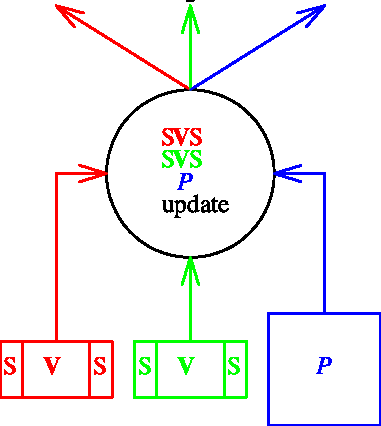
\includegraphics[width=10cm]{../pics/fvpups}}
\caption{Tight-coupled update of $3$~different species indicated by the different colours.
The first two species have a fluid representation consisting of two scalar fields
of density and temperature, and a velocity vector field. The third species~$P$
consists of particles. 
\label{fig:tight}}
\end{figure}

The natural alternative is loose-coupling, where not only is the ordering
\begin{equation} \label{eq:loose}
f_1,f_2,f_3,\ldots, g_1,g_2,g_3,\ldots,h_1,h_2,h_3,\ldots\ldots
\end{equation}
but separate smaller linear systems $A_f {\bf f}= {\bf b}_f$, 
$A_g {\bf g}= {\bf b}_g$, $A_h {\bf h}= {\bf b}_h$, \ldots, are solved in turn,
see \Fig{loose}. It should be evident that the information about updated values
of $h_j$ does not feed into the  new~$f_j$ until there is another cycle 
of updates $A_f {\bf f}= {\bf b}_f$, and then only imperfectly
compared to the tight-coupled approached.


\begin{figure}
\centerline{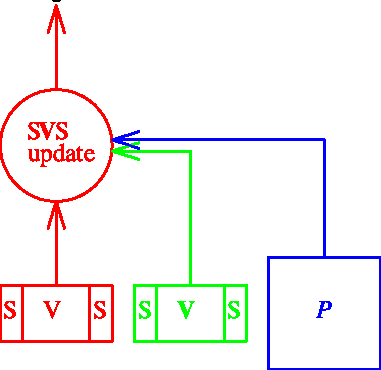
\includegraphics[width=6cm]{../pics/fvms}}
\centerline{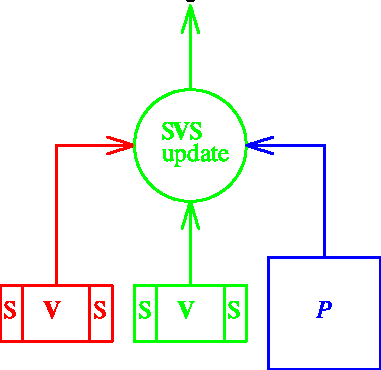
\includegraphics[width=6cm]{../pics/fvps}}
\centerline{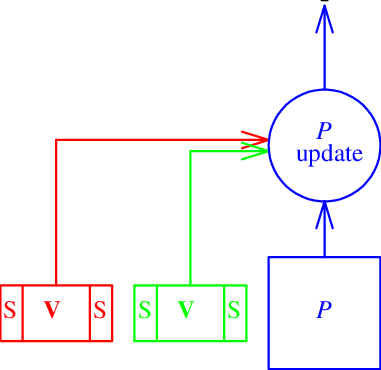
\includegraphics[width=6cm]{../pics/pups}}
\caption{Loose-coupled update of $3$~different species indicated by the different colours.
The first two species have a fluid representation consisting of two scalar fields
of density and temperature, and a velocity vector field. The third species~$P$
consists of particles.  As time increases down the page, first one fluid species
is updated, then the other, finally the particles are updated and the cycle repeats.
\label{fig:loose}}
\end{figure}

The matrix~$A$ will generally
be sparse, with most entries equal to zero, even when `static condensation'
as described in \Sec{sem} has been used to reduce the number of entries in~${\bf x}$
for Galerkin and to give HDG schemes. Since the finite elements will \emph{not} normally
be arranged in a regular pattern, the solution of the linear algebra
problem will have to be obtained by iteration.
These iterations are expected to benefit from appropriate matrix preconditioning, ie.\
algorithms which are mathematically equivalent to forming the 
matrix product $M=C^{-1}A$ so that $M{\bf x}=C^{-1}{\bf b}$ is easier to solve,
typically because iteration proceeds faster as $M$ is closer to a diagonal matrix.
Studies indicate that the balance between HDG and Galerkin
in terms of cost is so fine in classical hydrodynamics
that it is down to how the (reduced size) matrix problem is solved,
specifically the selection of preconditioner~$C$. %\cite{Ya16ToCG}.
Selection of preconditioners is generally regarded as an art.

Since finite elements are widely used in practical applications, much
research has been developed for the solution of the large, sparse
matrix problems which result. Local iterations, such as the Jacobi or Gauss-Seidel
typically taught in introductory courses, have rates of convergence limited
by the rate of information propagation just like the explicit schemes discussed above.
More efficient techniques are available such as (preconditioned) Conjugate Gradients,
which is `unreasonably effective' especially for the Poisson and similar
elliptic problems, and (preconditioned) Krylov methods of which GMRES is the
most popular for other types of physical model, see for example
van der Vorst's book. %~\cite{vandervorst}.
There are a number of practical considerations when it comes to implementing
these algorithms on computing hardware, particularly in relation to 
storage. Generally, forming the complete matrices such as~$A$ and $C^{-1}A$
is avoided as far possible, their entries may be only generated as required
and ideally only an algorithm specified for the action of the preconditioner.

Most attention has so far been paid to the solving the smaller subsystems
eg.\ $A_f {\bf f}= {\bf b}_f$ of the loose-coupling problem. Each can be
treated separately and the basic structures, vectors and sparse matrices of fixed size,
are features of most scientific packages and correspondingly often identified
by vendors for optimised implementation. In contrast,
solving the tight-coupled problem, especially where particle information is
involved, would benefit from further investigation.







